\documentclass[a4paper, 12pt, spanish]{article}

\usepackage[paper=a4paper, left=1.5cm, right=1.5cm, bottom=1.5cm, top=3.5cm]{geometry}
\usepackage[spanish, es-noshorthands]{babel}
\usepackage[utf8]{inputenc}
\usepackage[none]{hyphenat}
\usepackage[colorlinks,citecolor=black,filecolor=black,linkcolor=black,urlcolor=black]{hyperref}
\usepackage[table]{xcolor}
\usepackage{float}
\usepackage{caratula}
\usepackage{graphicx} 
\usepackage{fancyhdr}
\usepackage{lastpage}
\usepackage{caption}
\usepackage{subcaption}
\usepackage{multirow}
\usepackage{alltt}
\usepackage{tikz}
\usepackage{color}
\usepackage{gnuplottex}
\usepackage{verbatim}
\usepackage{framed}
\usepackage{amsmath}
\usepackage{amsfonts}
\usepackage{amssymb}
\usepackage{amsthm}
\usepackage[table]{xcolor}

% Acomodo fancyhdr.
\pagestyle{fancy}
\thispagestyle{fancy}
\addtolength{\headheight}{1pt}
\lhead{Teoría de las Comunicaciones}
\rhead{$2^{\mathrm{do}}$ cuatrimestre de 2015}
\cfoot{\thepage /\pageref*{LastPage}}
\renewcommand{\footrulewidth}{0.4pt}

\sloppy

\parskip=5pt % 10pt es el tama de fuente

% Pongo en 0 la distancia extra entre itemes.
\let\olditemize\itemize
\def\itemize{\olditemize\itemsep=0pt}


\materia{Teoría de las Comunicaciones}
\grupo{Conformación del grupo}
\tituloCaratula{Trabajo Práctico N$^\circ$2\\ \vspace{0.5cm} Rutas en Internet}

\integrante{Alvaro Jose Fernando}{89/10}{fer1578@gmail.com}
\integrante{Barbeito Nicolás}{147/10}{nicolasbarbeiton@gmail.com}
\integrante{Brum Raúl}{199/98}{brumraul@gmail.com}
\integrante{Nievas Yésica}{340/05}{yesica.nievas@gmail.com}



\begin{document}

%\setcounter{tocdepth}{2}

\begin{titlepage}

\maketitle

\end{titlepage}

\tableofcontents

\newpage
\section{Introducción}

En el presente trabajo nos propondremos analizar las diferentes rutas que siguen los paquetes IP en internet desde un host origen hasta alcanzar su host destino.\\
Para ello implementaremos una serie de herramientas basadas en el protocolo ``ICMP'' que nos permitan emular un ``traceroute'' al host destino.\\
Como objetivo adicional trataremos con esta herramienta poder detectar cuando un paquete pasa por un enlace submarino para lo cuál implementaremos un test de hipótesis que nos permita detectar estos enlaces y posteriormente compararemos los resultados obtenidos con la realidad.\\\\
Para cumplir con estos objetivos correremos una serie de test sobre hosts de distintas universidades, concretamente analizaremos los siguientes casos de estudio:

\begin{itemize}
\item[$\bullet$] \textbf{Tokyo:} University of Tokyo. Tokyo, Japon.
\item[$\bullet$] \textbf{Pretoria:} University of Pretoria. Pretoria, Sudáfrica.
\item[$\bullet$] \textbf{Málaga:} Universidad de Málaga. Málaga, España.
\item[$\bullet$] \textbf{MIT:} Massachusetts Institute of Technology. Cambridge, Estados Unidos
\end{itemize}

\section{Desarrollo} 

\section{Resultados y Análisis}
En esta sección presentaremos y analizaremos los resultados obtenidos al correr los distintos test propuestos.
Para ello correremos los mismos con una iteración de 100 repeticiones sobre los host de las siguientes universidades.

\subsection{Universidad de Tokyo}
El host de destino de la universidad de Tokyo sera el dominio ``www.u-tokyo.ac.jp'' cuya IP es ``210.152.135.178''. El host de la universidad de Tokyo se encuentra ubicado la ciudad de Tokyo, Japón. El origen sera un host ubicado en la Ciudad de Buenos Aires, Argentina utilizando como isp a Telecentro.

\subsubsection{Datos}

Los datos obtenidos para este caso fueron los siguientes:

\begin{table}[H]
    \begin{center}
        \begin{tabular}{| r | r | r | r | r |}
  \hline
  {\bf TTL} & \multicolumn{1}{|c|}{\bf IP} & {\bf E(RTT) (ms)} & {\bf S(RTT) (ms)} & {\bf $\Delta$RTT (ms)}\\
  \hline
\hline 1  & 192.168.10.1 & 0.414 & 0.025 & 0.414\\
\hline 2  & 10.20.64.1 & 9.588 & 2.179 & 9.174\\
\hline 3  & 200.115.194.173 & 9.709 & 2.050 & 0.121\\
\hline 4  & 208.178.195.210 & 11.823 & 2.660 & 2.114\\
\hline 5  & 208.178.195.209 & 10.154 & 3.919 & 0.000\\
\rowcolor{blue!25}\hline 6  & 64.212.107.98 & 140.102 & 2.736 & 129.948\\
\hline 7  & 129.250.3.172 & 141.972 & 6.459 & 1.870\\
\hline 8  & 129.250.2.219 & 165.020 & 5.163 & 23.048\\
\hline 9  & 129.250.7.69 & 174.848 & 10.839 & 9.828\\
\rowcolor{blue!25}\hline 10  & 129.250.2.177 & 289.040 & 10.215 & 114.191\\
\hline 11  & 129.250.6.144 & 286.955 & 9.046 & 0.000\\
\hline 12  & 61.200.80.218 & 281.767 & 6.327 & 0.000\\
\hline 13  & 158.205.192.173 & 287.145 & 8.005 & 5.378\\
\hline 14  & 158.205.192.86 & 300.318 & 5.018 & 13.173\\
\hline 15  & 158.205.121.250 & 299.293 & 22.325 & 0.000\\
\hline 16  & 154.34.240.254 & 287.327 & 2.431 & 0.000\\
\hline 17  & 210.152.135.178 & 300.554 & 3.888 & 13.227\\
\hline
        \end{tabular}
        \caption{$\overline{RTT}$, $\sigma$RTT y $\Delta$RTT para la ruta utilizada para llegar www.u-tokyo.ac.jp}
        \label{table:tokyo} 
    \end{center}
\end{table}

Analizando la información aportada por la tabla \ref{table:tokyo} podemos notar que tanto el salto 6 como 10 sobresalen por sobre el resto en cuanto a sus tiempos de $\Delta$RTT. 

\subsubsection{RTT y $\Delta$RTT}

\begin{figure}[H]
    \begin{center}
        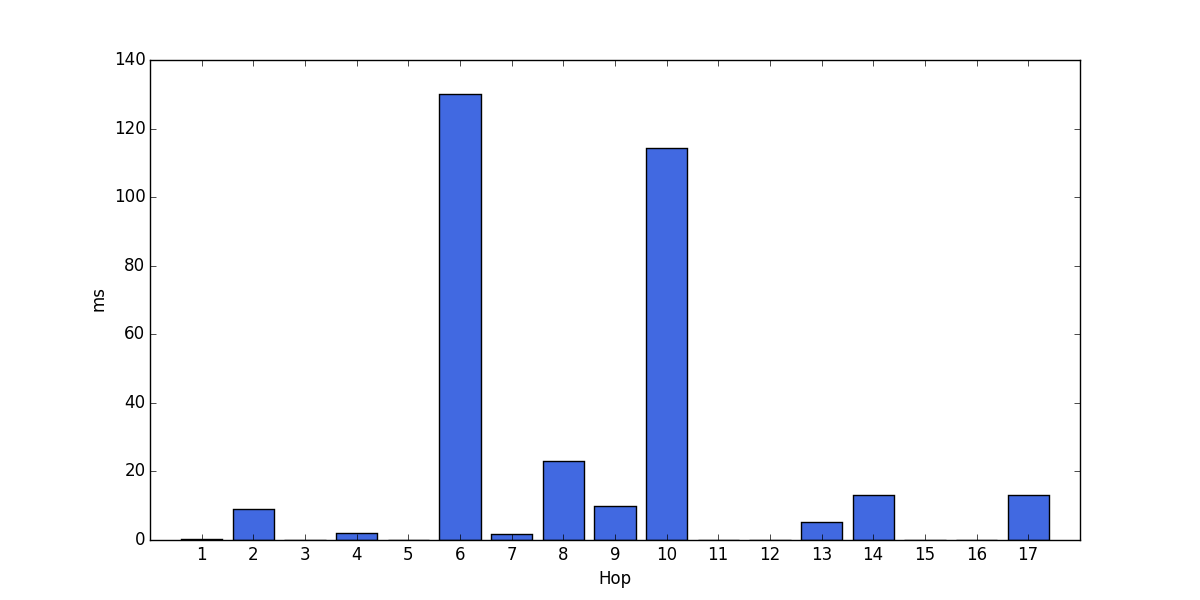
\includegraphics[width=1\textwidth]{data/rtt-tokyo-bar.png}
        \caption{www.u-tokyo.ac.jp - $\Delta$RTT}
        \label{histo:tokyo}
    \end{center}
\end{figure}

\begin{figure}[H]
    \begin{center}
        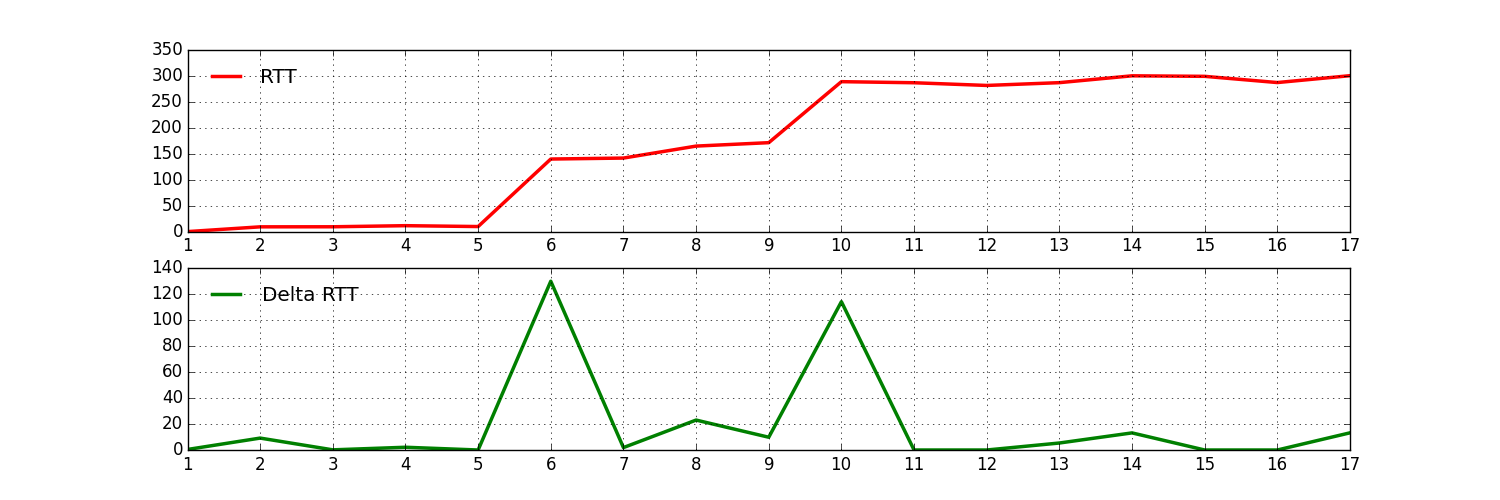
\includegraphics[width=1\textwidth]{data/rtt-tokyo-lines.png}
        \caption{www.u-tokyo.ac.jp - RTT y $\Delta$RTT}
        \label{lines:tokyo}
    \end{center}
\end{figure}

Tanto en la figura \ref{histo:tokyo} como en la figura \ref{lines:tokyo} podemos comprobar los que habíamos notado en la tabla \ref{table:tokyo}. Esto es que tanto el salto 6 como 10 se destacan por sobre el resto. En caso de existir algún enlace submarino seguramente este se correspondería con alguno de estos saltos. Esto lo analizaremos en las siguientes secciones.

\subsubsection{Test de Grubbs}\label{tokyo:grubbs}

\subsubsection{Geolocalización}

\begin{table}[H]
    \begin{center}
        \begin{tabular}{| r | r | c | c |}
  \hline
  {\bf TTL} & \multicolumn{1}{|c|}{\bf IP} & {\bf DNS} & {\bf Ubicación}\\
  \hline
\hline 1  & 192.168.10.1 & rig0.tuxhome.com.ar(ip privada) &\\
\hline 2  & 10.20.64.1 & no disponible(ip privada) &\\
\hline 3  & 200.115.194.173 & cpe-200-115-194-173.telecentro-reversos.com.ar & Buenos Aires, Argentina\\
\hline 4  & 208.178.195.210 & global-crossing-argentina-s-a.xe-0-1-0.ar3... & Buenos Aires, Argentina \\
\hline 5  & 208.178.195.209 & xe-0-1-0.ar3.eze1.gblx.net & Buenos Aires, Argentina \\
\rowcolor{blue!25}\hline 6  & 64.212.107.98 & no disponible  & Los Angeles, Usa\\
\hline 7  & 129.250.3.172 & ae-4.r21.miamfl02.us.bb.gin.ntt.net & Miami, Usa \\
\hline 8  & 129.250.2.219 & ae-4.r22.dllstx09.us.bb.gin.ntt.net & Dallas, Usa\\
\hline 9  & 129.250.7.69 & ae-5.r22.lsanca07.us.bb.gin.ntt.net & Los Angeles, Usa\\
\rowcolor{blue!25}\hline 10  & 129.250.2.177 & ae-0.r21.osakjp02.jp.bb.gin.ntt.net & Houston, Usa\\
\hline 11  & 129.250.6.144 & ae-5.r23.osakjp02.jp.bb.gin.ntt.net & Osaka, Japan\\
\hline 12  & 61.200.80.218 & xe-1-1-10.r23.osakjp02.jp.ce.gin.ntt.net & Osaka, Japan\\
\hline 13  & 158.205.192.173 & ae0.ostcr01.idc.jp & Tokyo, Japan\\
\hline 14  & 158.205.192.86 & no disponible  & Tokyo, Japan\\
\hline 15  & 158.205.121.250 & po2.l321.fk1.eg.idc.jp & Tokyo, Japan\\
\hline 16  & 154.34.240.254 & no disponible & Tokyo, Japan\\
\hline 17  & 210.152.135.178 & www.u-tokyo.ac.jp & Tokyo, Japan\\
\hline
        \end{tabular}
        \caption{Ruta utilizada para llegar www.u-tokyo.ac.jp con la ubicación de los diferentes saltos por los que se pasa. Se encuentran resaltados los saltos distiguidos calculados en la seccion \ref{tokyo:grubbs}}
        \label{table:tokyo} 
    \end{center}
\end{table}


\subsection{Universidad de Pretoria}
El host de destino de la universidad de Pretoria sera el dominio ``www.up.ac.za'' cuya IP es ``5.10.110.85''. El host de la universidad de Pretoria se encuentra ubicado la ciudad de Pretoria, en sudáfrica. El origen es un host ubicado en la Ciudad de Buenos Aires, Argentina utilizando como isp a Telecentro.

\subsubsection{Datos}

Los datos obtenidos para este caso fueron los siguientes:

\begin{table}[H]
    \begin{center}
        \begin{tabular}{| r | r | r | r | r |}
  \hline
  {\bf TTL} & \multicolumn{1}{|c|}{\bf IP} & {\bf E(RTT) (ms)} & {\bf S(RTT) (ms)} & {\bf $\Delta$RTT (ms)}\\
  \hline 
\hline 1  & 192.168.0.1 &  3.037 & 3.218 & 3.037\\
\rowcolor{blue!25}\hline 2  & 10.19.0.1 & 21.794 & 23.114 & 18.757\\
\hline 3  & 200.115.195.81 & 19.089 & 14.663 & 0.000\\
\hline 4  & 208.178.195.214 & 20.840 & 13.042 & 1.751\\ 
\hline 5  & 208.178.195.213 & 22.422 & 18.565 & 1.582\\ 
\rowcolor{blue!25}\hline 6  & 67.17.75.66 & 158.745 & 28.768 & 136.323\\ 
\hline 7  & 4.68.111.121 &  152.379 & 26.292 & 0.000\\ 
\rowcolor{blue!25}\hline 8  & 4.69.168.11 & 272.512 & 19.879 & 120.133\\ 
\hline 9  & 4.69.168.11 & 277.326 & 26.226 & 4.814\\ 
\rowcolor{blue!25}\hline 10  & 212.73.206.174 & 292.420 & 28.952 & 15.094\\ 
\hline 11  & 50.97.19.101 & 281.778 & 31.841 & 0.000\\ 
\hline 12  & 50.97.19.41 & 289.224 & 33.909 & 7.446\\ 
\hline 13  & 5.10.118.135 & 278.807 & 23.145 & 0.000\\ 
\hline 14  & 5.10.110.85 & 279.282 & 18.527 & 0.476\\ 
\hline
        \end{tabular}
        \caption{$\overline{RTT}$, $\sigma$RTT y $\Delta$RTT para la ruta utilizada para llegar www.up.ac.za}
        \label{table:pretoria} 
    \end{center}
\end{table}

Analizando la información aportada por la tabla \ref{table:pretoria} podemos notar que los saltos 2, 6, 8 y 10 sobresalen por sobre el resto en cuanto a sus tiempos de $\Delta$RTT. 

\subsubsection{RTT y $\Delta$RTT}

\begin{figure}[H]
    \begin{center}
        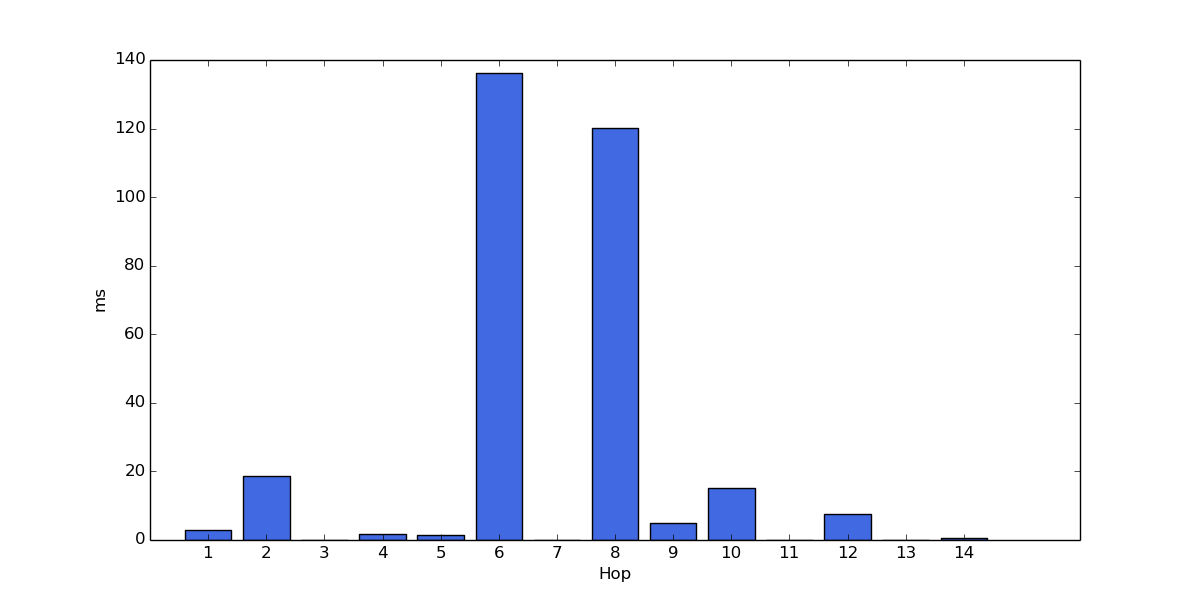
\includegraphics[width=1\textwidth]{data/rtt-pretoria-bar.png}
        \caption{www.up.ac.za - $\Delta$RTT}
        \label{histo:pretoria}
    \end{center}
\end{figure}

\begin{figure}[H]
    \begin{center}
        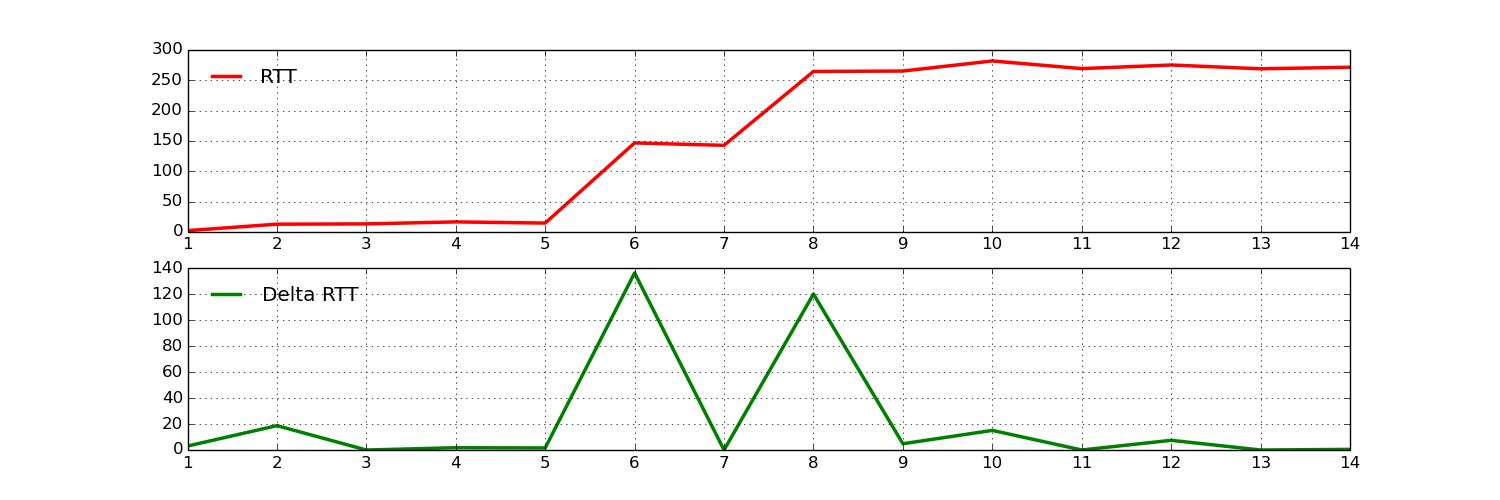
\includegraphics[width=1\textwidth]{data/rtt-pretoria-lines.png}
        \caption{www.up.ac.za - RTT y $\Delta$RTT}
        \label{lines:pretoria}
    \end{center}
\end{figure}

Tanto en la figura \ref{histo:pretoria} como en la figura \ref{lines:pretoria} podemos comprobar los que habíamos notado en la tabla \ref{table:pretoria}. Esto es que tanto los saltos 2, 6, 8 y 10 se destacan por sobre el resto. En caso de existir algún enlace submarino seguramente este se correspondería con alguno de estos saltos. Esto lo analizaremos en las siguientes secciones.

\subsubsection{Test de Grubbs}\label{pretoria:grubbs}

\subsubsection{Geolocalización}

\begin{table}[H]
    \begin{center}
        \begin{tabular}{| r | r | c | c |}
  \hline
  {\bf TTL} & \multicolumn{1}{|c|}{\bf IP} & {\bf DNS} & {\bf Ubicación}\\
  \hline
\hline 1  & 192.168.0.1 & (ip privada) & \\
\rowcolor{blue!25}\hline 2  & 10.19.0.1 & (ip privada) & \\
\hline 3  & 200.115.195.81 & cpe-200-115-195-81.telecentro-reversos.com.ar & Buenos Aires, Argentina\\
\hline 4  & 208.178.195.214 & global-crossing-argentina-s-a.xe-0-3-1.ar3.eze1.gblx.net & Virginia, USA\\ 
\hline 5  & 208.178.195.213 & xe-0-3-1.ar3.eze1.gblx.net & Virginia, USA\\ 
\rowcolor{blue!25}\hline 6  & 67.17.75.66 &  po3-20G.ar3.MIA2.gblx.net & Miami, USA\\ 
\hline 7  & 4.68.111.121 &  ae5.edge2.miami2.level3.net  & Miami, USA\\ 
\rowcolor{blue!25}\hline 8  & 4.69.168.11 & ae-1-60.ear1.Paris1.Level3.net & Paris, Francia\\ 
\hline 9  & 4.69.168.11 & ae-1-60.ear1.Paris1.Level3.net & Paris, Francia\\ 
\rowcolor{blue!25}\hline 10  & 212.73.206.174 & unknown.Level3.net & Los Angeles, USA\\ 
\hline 11  & 50.97.19.101 & ae1.bbr02.tg01.lon01.networklayer.com & Londres, Inglaterra\\ 
\hline 12  & 50.97.19.41 & ae6.dar01.lon02.networklayer.com & Londres, Inglaterra\\ 
\hline 13  & 5.10.118.135 & po1.fcr01b.lon02.networklayer.com & Londres, Inglaterra\\ 
\hline 14  & 5.10.110.85 &  55.6e.0a05.ip4.static.sl-reverse.com & Londres, Inglaterra\\ 
\hline
        \end{tabular}
        \caption{Ruta utilizada para llegar www.up.ac.za con la ubicación de los diferentes saltos por los que se pasa. Se encuentran resaltados los saltos distiguidos calculados en la seccion \ref{pretoria:grubbs}}
        \label{table:pretoria} 
    \end{center}
\end{table}

\section{Conclusiones}

Tras haber corrido los distintos test sobre los host bajo estudio notamos que no obtuvimos variaciones en las rutas utilizadas por los paquetes, sino que generalmente se mantuvieron las mismas rutas entre las distintas corridas. 
Notamos también que la información provista por los servicios de geolocalización en muchos casos no se se corresponde con la localización física del router.
En cuanto a la localización de enlaces submarinos mediante el test de hipótesis realizado en los cuatro casos de estudio el mismo detecto en forma correcta los mismos por lo cuál concluimos que el uso de esta herramienta podría llegar a ser viable para la detección de los mismos.
Otra particularidad que notamos es que muchos routers asignan una menor prioridad a los paquetes ``ICMP'' lo que origino que varios saltos tuviesen $\Delta$RTT negativos.

A continuación expondremos las particularidades de cada caso de estudio:

\subsection{Universidad de Tokyo}

Para este caso de estudio mas allá del error informado por los servicios de geolocalización para el salto 10 de la tabla de la figura \ref{table:tokyo}, tanto los valores de RTT obtenidos como los outliers detectados por el test de Grubbs parecen tener correspondencia con lo realmente acontecido.\\
Si bien los $\Delta$RTT obtenidos parecen no seguir una distribución normal los outliers obtenidos mediante el test de Grubbs para detectar los enlaces submarinos parecen ser los correctos y coinciden con lo que se puede apreciar en los gráficos de las figura \ref{histo:tokyo} y la figura \ref{lines:tokyo}.

\subsection{Universidad de Pretoria}

\subsection{Universidad de Málaga}

\subsection{Universidad MIT}


\ref{LastPage}

\end{document}
